\documentclass[a4paper,10pt,twoside]{article}
%%%%%%%%%%% Packages %%%%%%%%%%
\usepackage[margin=1in]{geometry}
\usepackage{amsmath, amssymb,mathtools}
\usepackage{fancyhdr}
\usepackage{sectsty}
\usepackage{graphicx,wrapfig}
\usepackage{enumitem}
\usepackage{float}
\usepackage{braket}
\usepackage{bbm}
\usepackage{tikz,calc}
\usepackage{amsthm}


%%%%%%%%%%% Macros %%%%%%%%%%
\def \note#1 {\vspace{-1em}\paragraph{\bfseries #1}}
\def \dd {{\rm d}}
\def \id {{\mathbbm{1}}}
\def \order {\mathcal{O}}
\def\bquad{\mkern-18mu}
\DeclareMathOperator{\trace}{tr}
\DeclareMathOperator{\spanset}{span}

%%%%%%%%%%% Tikz Definitions %%%%%%%%%%
\usetikzlibrary{shapes, arrows,positioning,fit}
\tikzstyle{plain} = [draw,thick,circle,inner sep=0,minimum size=0.5cm,font=\footnotesize]
\tikzstyle{mps} = [draw,thick,rectangle,rounded corners=.1cm,inner sep=0,minimum size=0.5cm]
\tikzstyle{mpo} = [draw,thick,circle,inner sep=0,minimum size=0.5cm]
\tikzstyle{index} = [-,thick,font=\footnotesize]
\tikzstyle{virtual} = [-,thick,dotted,font=\footnotesize]

\def \tu {0.25cm}

%%%%%%%%%%% Formatting %%%%%%%%%%
\pagestyle{fancy}
\renewcommand{\footrulewidth}{0.5pt}

\fancyhf{}
\lhead{18/05/2017}
\chead{Quantum Information Methods in Many-Body Physics}
\rhead{PH2269}
\lfoot{Giacomo Giudice~~~~giacomo.giudice@mpq.mpg.de}
\rfoot{Page \thepage}

\allsectionsfont{\normalfont\sffamily}

\newtheoremstyle{modern}{3pt}{3pt}{\itshape}{}{\sffamily\bfseries}{}{.5em}{}
\theoremstyle{modern}
\newtheorem{lemma}{Lemma}[section]
\newtheorem{theorem}[lemma]{Theorem}

%%%%%%%%%%% Here Begins Document %%%%%%%%%%
\begin{document}
\title{\vspace{-1cm}\sffamily Solutions to Homework 5\vspace{-1cm}}
\author{}
\date{}
\maketitle
\thispagestyle{fancy}

\begin{section}{}
The only two terms one may suspect not to commute are an adjacent vertex term and plaquette term. 
However, since any given vertex and plaquette share an even number of edges, the minus signs arising from the commutation of $X$ and $Z$ cancel out.
\begin{align*}
  A_v \ket{\Psi^0} &= \prod_p \frac{1}{\sqrt{2}} \left(\id + B_p\right) \underbrace{A_v \ket{0}^{\otimes N}}_{=\ket{0}^{\otimes N}} = \ket{\Psi^0} , \\
  B_p \ket{\Psi^0} &= \frac{1}{\sqrt{2}} \left(B_p + \id \right)\prod_{p^\prime \neq p} \frac{1}{\sqrt{2}} \left(\id + B_{p^\prime}\right) \ket{0}^{\otimes N} = \ket{\Psi^0} .
\end{align*}
Therefore $\ket{\Psi^0}$ is an eigenvalue for each $A_v$, $B_p$.
Since the spectrum of these operators is $\{+1,-1\}$, it corresponds to the eigenvector of $H$ with the smallest eigenvalue:  $H \ket{\Psi^0} = -2N \ket{\Psi^0}$.

In the style of a binomial expansion, the state $\ket{\Psi^0}$ can be rewritten as a sum of an increasing number of plaquettes.
Notice that adjacent plaquettes cancel out their effect on the bulk, i.e. they only flip spins on the boundary, which is a closed path.
Therefore the state corresponds to the equally weighted sum of all possible ``loop'' configurations.
Informally
\[
   \ket{\Psi^0} = \frac{1}{\sqrt{\rm norm}}\sum_{\rm loop} \ket{\rm loop},
\]
where by $\ket{\rm loop}$  we mean the state which has a configuration of $\ket{1}$ on the edges such that there are no endpoints.

Notice that $[\hat{X}_{1,2},A_v] =  [\hat{X}_{1,2},B_p] = 0$. 
Therefore
\[
  \ket{\Psi^0_{ij}} = \prod_p \frac{1}{\sqrt{2}} \left(\id + B_p\right) \hat{X}_1^i \hat{X}_2^j \ket{0}^{\otimes N},
\]
from which the different $\ket{\Psi_{ij}^0}$ are clearly eigenvectors of $H$ (using the previous argument) and are orthogonal.

The plaquette operations can transform any loop configuration down to one of the $\hat{X}_1^i \hat{X}_2^j \ket{0}^{\otimes N}$.
However a state $\hat{X}_{1,2}\ket{0}^{\otimes N}$ cannot be reduced to the vacuum state.
One can see this by considering that the $B_v$ operations always spin an equal number of flips on every vertical and horizontal direction.
Therefore we can write 
\[
  \ket{\Psi_{ij}^0} = \frac{1}{\sqrt{\rm norm}}\sum_{\mathclap{{\rm loop} \left| \substack{\#_1 = i \\ \#_2 = j } \right. }}  \ \ket{\rm loop} .
\]
This can be formalized a bit more by defining the operators
\[
  \hat{Z}_{1,2} = \prod_{j \in l_{1,2}} Z_j
\]
Notice that for any loop configuration, this operator gives $\pm 1$, independent of where the loop is placed.
We can label then the parity of the different ground states, since $ \braket{\Psi_{ij}^0 | \hat{Z}_{1,2} | \Psi_{ij}^0} = (-1)^i (-1)^j$.
\end{section}

\begin{section}{}
Let us consider first $W_l^{(e)}$.
This operator commutes with the plaquette operator, and with all the vertex operators $A_v$, except for the end-points $s_1$ and $s_2$.
At these points only one edge overlaps, and we have $W_l^{(e)} A_{s_1} = - A_{s_1} W_l^{(e)}$, since $XZ = -ZX$.
When applying $H$ to $\ket{\Psi_{s_1,s_2}^{(e)}}$, we get two $+1$ contributions by pulling through the $W_l^{(e)}$.
Hence, $H\ket{\Psi_{s_1,s_2}^{(e)}} = -2(N-2)\ket{\Psi_{s_1,s_2}^{(e)}}$.

Analogously, the $W_{l^*}^{(m)}$ commutes with everything except the plaquettes at the end-points $p_1$ and $p_2$, which anticommute.
Therefore $W_{l^*}^{(m)}$ creates two quasi-particles at an energy cost of $+2$ each.
\end{section}

\begin{section}{}
In order to check the statistics, we must look at the phase it obtains under exchange of the particles.
For both bosons and fermions, two exchanges (i.e. a full rotation of one particle around the other) leaves the state unchanged.
One can check that the self-statistics of two $\psi$ is fermionic,  by expliticly moving one $\psi$ around one other.
Kitaev and Laumann\footnote{A. Kitaev, C. Laumann, Lecture Notes from Les Houches Summer School (2009) arXiv:0904.2771.} propose another argument. 
In the lecture we saw that the $e$ and $m$ excitations behave as bosons, while their mutual statistics is anyonic.
Schematically
\begin{figure}[h]
  \centerline{
    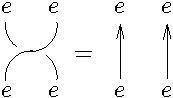
\includegraphics[width=0.2\textwidth]{img/eq-exch-ee.pdf}\hspace{2em}
    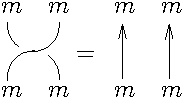
\includegraphics[width=0.2\textwidth]{img/eq-exch-mm.pdf}
  }
\end{figure}
\begin{figure}[h]
  \centerline{
    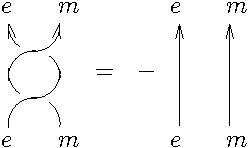
\includegraphics[width=0.25\textwidth]{img/eq-mutual-em.pdf}
  }
\end{figure}

Therefore,
\begin{figure}[h]
  \centerline{
    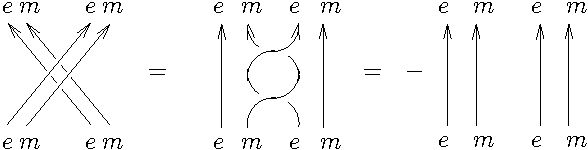
\includegraphics[width=0.6\textwidth]{img/eq-exch-emem.pdf}
  }
\end{figure}

\end{section}

\begin{section}{}
In addition to the two loops around the torus, there are two additional loops that are not contractible.
These loops are those around the holes. 
Hence, there are a total of $2^{2+2}=16$ ground states.
\note{Bonus}  Yes, as one can check by rotating one of the holes around the torus\footnote{E.B. Burger, M. Starbird, \emph{The heart of mathematics: an invitation to effective thinking} (2004).}.
\end{section}
\end{document}
%%%%%%%%%%% Here Ends Document %%%%%%%%%%
